 \documentclass[conference]{IEEEtran}
\usepackage[utf8]{inputenc}
\usepackage{textcomp}
\usepackage[spanish]{babel}
\usepackage{amsmath}
\usepackage{amsfonts}
\usepackage{amssymb}
%Dependencies for [1.]
\usepackage{enumerate}
%Dependencies for [1.]
\usepackage{graphicx}
%\usepackage{xcolor}
% Dependencies for Excel2Latex
\usepackage[table]{xcolor}
\usepackage{booktabs}
% Dependencies for Excel2Latex
\usepackage{listings}
\usepackage{tikz}
\usepackage{float}
\usepackage{karnaugh-map}
\usepackage{adjustbox}
\usepackage[left=1cm,right=1cm,top=1cm,bottom=1cm]{geometry}

%Habilita bookmarks en PDF
\newcommand\MYhyperrefoptions{bookmarks=true,bookmarksnumbered=true,
pdfpagemode={UseOutlines},plainpages=false,pdfpagelabels=true,
colorlinks=true,linkcolor={black},citecolor={black},
urlcolor={blue}}
\usepackage[\MYhyperrefoptions]{hyperref}
%Habilita bookmarks en PDF

% Dependencies for code blocks
% More info in https://en.wikibooks.org/wiki/LaTeX/Source_Code_Listings
\usepackage{listings}

\lstdefinestyle{CMD_small}
{
    backgroundcolor=\color{black},
    basicstyle=\tiny\color{white}\ttfamily,
    breaklines=true,
    postbreak=\mbox{\textcolor{red}{$\hookrightarrow$}\space},
    keywordstyle=\textcolor{red},
    morekeywords={pip, echo, if, ERRORLEVEL}
}

% Dependencies for code blocks

%Titulo del documento
\title{Proyecto Final de Investigación: Avance 1}

\makeatletter
\newcommand{\linebreakand}{%
  \end{@IEEEauthorhalign}
  \hfill\mbox{}\par
  \mbox{}\hfill\begin{@IEEEauthorhalign} \hfill
}
\makeatother

\renewcommand\thesection{\arabic{section}}
\renewcommand\thesubsection{\thesection.\arabic{subsection}}
\renewcommand\thesubsubsection{\thesubsection.\arabic{subsubsection}}

\author{
	\IEEEauthorblockN{Chavarria Peña Jonathan Andrés}
	\IEEEauthorblockA{\textit{Estudiante Ing. en Sistemas de Computación}\\ 
	\textit{Universidad Fidélitas}\\
	San José, Costa Rica \\
	\href{mailto:jonach1998@gmail.com}{jonach1998@gmail.com}}
\and
	\IEEEauthorblockN{Morales Cordero Valeria}
	\IEEEauthorblockA{\textit{Estudiante Ing. en Sistemas de Computación}\\ 
	\textit{Universidad Fidélitas}\\
	San José, Costa Rica \\
	\href{mailto:valemc0603@gmail.com}{valemc0603@gmail.com}}
\linebreakand % <------------- \and with a line-break
	\IEEEauthorblockN{Phillips Tencio Edmond\hfill}
	\IEEEauthorblockA{\textit{Estudiante Ing. en Sistemas de Computación}\\
	\textit{Universidad Fidélitas}\\
	Alajuela, Costa Rica \\
	\href{mailto:ephillips10986@ufide.ac}{ephillips10986@ufide.ac}}
\and
	\IEEEauthorblockN{Sánchez Camacho Carlos Daniel} 
	\IEEEauthorblockA{\textit{Estudiante Ing. en Sistemas de Computación}\\
	\textit{Universidad Fidélitas}\\
	San José, Costa Rica \\
	\href{mailto:csanchez20965@ufide.ac}{csanchez20965@ufide.ac}}

}


%Inicio del documento
\begin{document}

\maketitle

%Agrega numeracion a las paginas
%\thispagestyle{plain}
%\pagestyle{plain}

%\begin{abstract}

	
%\end{abstract}


\section{DESARROLLO}

\section{Investigación de la tecnología}

\subsection{Unit Testing}

En el siguiente proyecto se realizarán pruebas a un programa, las mismas se harán utilizando unit testing; pero para poder utilizarlo es importante comprender qué es y cómo utilizarlo. El unit test se define, como el código necesario para comprobar que el código del programa principal esté funcionando como esperábamos. Los unit test son una de muchas pruebas que se pueden realizar para comprobar que los programas estén en funcionamiento.
Los unit test se conforman de pequeños tests que comprueban que cada parte de los requisitos del código estén correctos; asimismo, se verifican sus resultados.
A la hora de realizar un unit test se puede dividir por partes especificas (Organizar, actuar y afirmar) cada “función” o “caso” que se va a realizar, estas son las siguiente:

\begin{itemize}
\item Arrange: Esta primera parte del caso a testear es donde se deben definir las variables o requisitos que necesita el programa para funcionar.
\item Act: Esta parte consiste en llamar a los métodos o funciones que se desean probar del código del programa principal a testear. 
\item Asert: En la última sección se prueba si los resultados son correctos o incorrectos. Dependiendo del resultado, si son correctos se valida y continúa con los otros casos, o se repara, no se continua hasta que el error desaparezca.
\end{itemize}

Estas partes pueden cambiar de nombre dependiendo de donde se investigue, otros nombres que reciben son Given, When, Then (Dado que, cuando, entonces).
Para la última parte del caso (Asert o Then), si hay errores de integración es necesario investigar si se necesitan otros tipos de pruebas de software y de esta manera lograr comprobar la efectividad total del código.
Al hacer unit testing se asegura que cada parte el código esta bien y es útil. Es importante saber que los fallos y errores son inevitables, por esto mismo los unit test no se pueden considerar como opcionales. Ya que una aplicación, sitio web, programa o código sin pruebas se puede considerar como inestable, voluble o deficiente.
Las pruebas pueden ser desarrolladas por los desarrolladores, mismos que conocen bien el código o también en muchas empresas también las pueden realizar los responsables de QA.

\section{Software a utilizar}

El software a utilizar en la presente investigación es Python -m unittes, es el módulo unittest, este ofrece la posibilidad de crear las pruebas implementando una clase llamada unittest.TestCase en la que se incluirán métodos de pruebas. Tales como los siguientes: 

% Table generated by Excel2LaTeX from sheet 'Hoja1'
\begin{table}[H]
  \centering
  \caption{Métodos de unittest.}
    \begin{tabular}{|p{10.335em}|p{6.28em}|p{4em}|}
    \toprule
    \rowcolor[rgb]{ .933,  .933,  .933} \textcolor[rgb]{ .133,  .133,  .133}{\textbf{Method}} & \textcolor[rgb]{ .133,  .133,  .133}{\textbf{Checks that}} & \textcolor[rgb]{ .133,  .133,  .133}{\textbf{New in}} \\
    \midrule
    \textcolor[rgb]{ .02,  .388,  .757}{assertEqual(a, b)} & \textcolor[rgb]{ .133,  .133,  .133}{a == b} & \multicolumn{1}{l|}{\textcolor[rgb]{ .133,  .133,  .133}{}} \\
    \midrule
    \textcolor[rgb]{ .02,  .388,  .757}{assertNotEqual(a, b)} & \textcolor[rgb]{ .133,  .133,  .133}{a != b} & \multicolumn{1}{l|}{\textcolor[rgb]{ .133,  .133,  .133}{}} \\
    \midrule
    \textcolor[rgb]{ .02,  .388,  .757}{assertTrue(x)} & \textcolor[rgb]{ .133,  .133,  .133}{bool(x) is True} & \multicolumn{1}{l|}{\textcolor[rgb]{ .133,  .133,  .133}{}} \\
    \midrule
    \textcolor[rgb]{ .02,  .388,  .757}{assertFalse(x)} & \textcolor[rgb]{ .133,  .133,  .133}{bool(x) is False} & \multicolumn{1}{l|}{\textcolor[rgb]{ .133,  .133,  .133}{}} \\
    \midrule
    \textcolor[rgb]{ .02,  .388,  .757}{assertIs(a, b)} & \textcolor[rgb]{ .133,  .133,  .133}{a is b} & \textcolor[rgb]{ .133,  .133,  .133}{3.1} \\
    \midrule
    \textcolor[rgb]{ .02,  .388,  .757}{assertIsNot(a, b)} & \textcolor[rgb]{ .133,  .133,  .133}{a is not b} & \textcolor[rgb]{ .133,  .133,  .133}{3.1} \\
    \midrule
    \textcolor[rgb]{ .02,  .388,  .757}{assertIsNone(x)} & \textcolor[rgb]{ .133,  .133,  .133}{x is None} & \textcolor[rgb]{ .133,  .133,  .133}{3.1} \\
    \midrule
    \textcolor[rgb]{ .02,  .388,  .757}{assertIsNotNone(x)} & \textcolor[rgb]{ .133,  .133,  .133}{x is not None} & \textcolor[rgb]{ .133,  .133,  .133}{3.1} \\
    \midrule
    \textcolor[rgb]{ .02,  .388,  .757}{assertIn(a, b)} & \textcolor[rgb]{ .133,  .133,  .133}{a in b} & \textcolor[rgb]{ .133,  .133,  .133}{3.1} \\
    \midrule
    \textcolor[rgb]{ .02,  .388,  .757}{assertNotIn(a, b)} & \textcolor[rgb]{ .133,  .133,  .133}{a not in b} & \textcolor[rgb]{ .133,  .133,  .133}{3.1} \\
    \midrule
    \textcolor[rgb]{ .02,  .388,  .757}{assertIsInstance(a, b)} & \textcolor[rgb]{ .133,  .133,  .133}{isinstance(a, b)} & \textcolor[rgb]{ .133,  .133,  .133}{3.2} \\
    \midrule
    \textcolor[rgb]{ .02,  .388,  .757}{assertNotIsInstance(a, b)} & \textcolor[rgb]{ .133,  .133,  .133}{not isinstance(a, b)} & \textcolor[rgb]{ .133,  .133,  .133}{3.2} \\
    \bottomrule
    \end{tabular}%
  \label{tab:addlabel}%
\end{table}%


El modulo de unit test de python permite utilizar distintos contenedores al realizar pruebas unitarias, como por ejemplo: list, dict y set.

Cada una de las pruebas puede devolver tres respuestas dependiendo del resultado, así como las siguientes:

\begin{itemize}
\item OK: Para mostrar que la prueba se ha completado con éxito.
\item FAIL: Para mostrar que la prueba no ha pasado exitosamente y se lanza una excepción como esta: AssertionError (sentencia verdadero-falso)
\item ERROR: Para dar a entender que la prueba no ha pasado exitosamente, pero el resultado en lugar de ser una aserción es un error.
\end{itemize}

Unittest.TestCase este incluye la cantidad de tiempo que tomaron las pruebas, junto con un indicador de estado para cada prueba. 

\subsection{Escritura de pruebas unitarias para el paquete test}

Se prefiere que las pruebas que utilizan el módulo unittest sigan algunas pautas. Una es nombrar el módulo de prueba comenzando con test y terminarlo con el nombre del módulo que se está probando. Los métodos de prueba en el módulo de prueba deben comenzar con test y terminar con una descripción de lo que el método está probando. Esto es necesario para que el controlador de prueba reconozca los métodos como métodos de prueba. Por lo tanto, no se debe incluir una cadena de caracteres de documentación para el método. Se debe usar un comentario (como Tests function returns only True or False) para proporcionar documentación para los métodos de prueba. Esto se hace porque las cadenas de documentación se imprimen si existen y, por lo tanto, no se indica qué prueba se está ejecutando.

\subsection{Plantilla básica para realizar unit test}

\begin{lstlisting}[language=Python,basicstyle=\scriptsize, breaklines=true,
    postbreak=\mbox{\textcolor{red}{$\hookrightarrow$}\space}]
import unittest
from test import support

class MyTestCase1(unittest.TestCase):

    # Only use setUp() and tearDown() if necessary

    def setUp(self):
        ... code to execute in preparation for tests ...

    def tearDown(self):
        ... code to execute to clean up after tests ...

    def test_feature_one(self):
        # Test feature one.
        ... testing code ...

    def test_feature_two(self):
        # Test feature two.
        ... testing code ...

    ... more test methods ...

class MyTestCase2(unittest.TestCase):
    ... same structure as MyTestCase1 ...

... more test classes ...

if __name__ == '__main__':
    unittest.main()

\end{lstlisting}


\section{Programa a probar}

El código al que se le realizarán pruebas será desarrollado en Python, este programa solicita al usuario que ingrese la cédula de la persona que desea buscar y la fecha de nacimiento de la misma, esta información se utilizará para encontrar los datos de la persona en una base de datos ya establecida. Al encontrar la información se imprime en pantalla la siguiente información: saludo, nombre completo, edad, centro de votación y los candidatos oficiales a presidencia y los posibles candidatos. Siendo esta ultima información recolectada desde Wikipedia. La base de datos estará ubicada en el mismo directorio raíz donde esta el programa, si este se borra o se le modifica el nombre, el programa no funcionará.

La idea de este programa es lograr proporcionar de manera fácil información para los votantes. Ya que fácilmente pueden conocer en que región deben votar y los actuales candidatos, además de posibles candidatos a presidencia.


\begin{lstlisting}[style=CMD_small]
C:\Python39\python.exe C:/git/calidad_software_proyecto/Proyecto_Final/Codigo/Votaciones.py
Favor ingrese su cedula sin guiones y con los 0 respectivos: 117110446
Favor ingresar su fecha de nacimiento en el formato dd/mm/yyyy: 13/06/1998
Hola JONATHAN ANDRES
Su nombre completo es: JONATHAN ANDRES CHAVARRIA PENA
Su edad es: 23
Su centro de votacion se ubica en:
	Provincia: SAN JOSE
	Canton: MONTES DE OCA
	Distrito: LOURDES
La lista de candidatos es la siguiente:
                       Partido                  Candidato    Tipo de candidato
0          Liberacion Nacional  Jose Maria Figueres Olsen    Candidato Oficial
1              Nueva Republica    Fabricio Alvarado Munoz    Candidato Oficial
3  Accesibilidad Sin Exclusion   oscar Andres Lopez Arias    Candidato Oficial
4             Accion Ciudadana   Marcia Gonzalez Aguiluz   **Posible Candidato
5             Accion Ciudadana  Carolina Hidalgo Herrera   **Posible Candidato
6             Accion Ciudadana     Welmer Ramos Gonzalez   **Posible Candidato
7             Accion Ciudadana     Hernan Solano Venegas   **Posible Candidato
8             Accion Ciudadana     Martha Zamora Castillo  **Posible Candidato
9        Movimiento Libertario    Carlos Valenciano Kamer    Candidato Oficial

Process finished with exit code 0
\end{lstlisting}

%\begin{figure}[H]
%\centering
%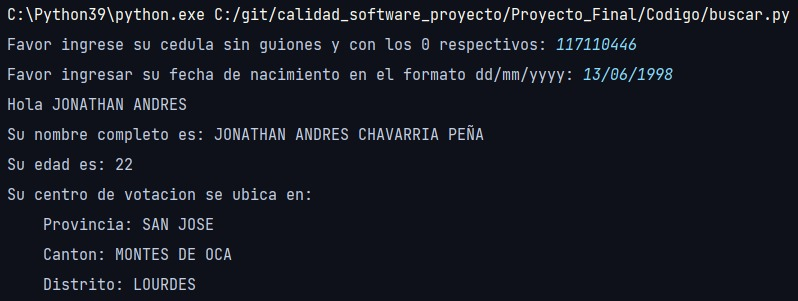
\includegraphics[scale=0.35]{imagenes/ejemplo_programa_a_probar.jpeg}
%\caption{Ejemplo de impresión del programa a probar.}
%\end{figure}


\section{Pruebas a realizar}

Para el proyecto necesitamos saber los casos específicos que vamos a probar en nuestro software por lo que definimos los siguientes:

\begin{enumerate}

\item Probar el caso en el que todo salga bien

\item Probar si la base de datos "Distelec.txt" tiene un formato incorrecto

\item Probar si la base de datos "PADRON\_COMPLETO.txt" tiene un formato incorrecto

\item Probar si se ingresa la cédula con letras o caracteres especiales.

\item Probar si no se encuentra una cedula en la base de datos

\item Probar si se deja alguno de los datos solicitados en blanco

\item Probar si no existe el archivo de la base de datos "Distelec.txt"

\item Probar si no existe el archivo de la base de datos "PADRON\_COMPLETO.txt"

\item Probar si la edad se ingreso en el formato correcto (prueba puede ser: mm/dd/yyyy)

\item Probar si la edad contiene letras o caracteres especiales

\item Probar si la pagina es incorrecta 

\item Probar si la pagina no se encuentra

\end{enumerate}


\section{Casos de prueba}

\subsection{Caso 1}
\begin{itemize}
\item Nombre/Identificador: Probar el caso en el que todo salga bien.
\item Descripción: El usuario digita bien toda la información.
\item Objetivo de la prueba: Comprobar el buen funcionamiento del programa.
\item Requerimientos o precondiciones: Estar incluido en la lista de votantes del país.
\item Pasos a seguir: 
\begin{enumerate}
\item Escribir la cédula, en el espacio correspondiente.
\item Escribir la fecha de nacimiento, en el espacio correspondiente.
\end{enumerate}
\item Resultados esperados: Despliegue de toda la información solicitada.
\item Prioridad: Alta
\item Datos a utilizar: 
\begin{itemize}
\item Cedula: 000000000
\item Fecha de nacimiento: 00/00/00
\end{itemize}
\item Tipo de prueba: Funcional
\end{itemize}

\subsection{Caso 2}
\begin{itemize}
\item Nombre/Identificador: Probar si la base de datos "Distelec.txt" tiene un formato incorrecto.
\item Descripción: Verificar que el archivo Distelec este separado por otro carácter que no sea comas.
\item Objetivo de la prueba: Comprobar que el programa falle cuando el archivo no esta separado por comas. 
\item Requerimientos o pre condiciones: Archivo en el formato incorrecto.
\item Pasos a seguir: 
\begin{enumerate}
\item Buscar el archivo "Distelec.txt" en la carpeta donde esta el programa.
\item Separar la información del archivo, utilizando como referencia la "," para separar.
\end{enumerate}
\item Resultados esperados: No se pueda correr el programa.
\item Prioridad: Alta
\item Datos a utilizar: 
\begin{itemize}
\item Archivo: "Distelec.txt"
\end{itemize}
\item Tipo de prueba: Funcional
\end{itemize}

\subsection{Caso 3}
\begin{itemize}
\item Nombre/Identificador: Probar si la base de datos "PADRON\_COMPLETO.txt" tiene un formato incorrecto.
\item Descripción: Verificar que el archivo PADRON\_COMPLETO este separado por otro carácter que no sea comas.
\item Objetivo de la prueba: Comprobar que el programa falle cuando el archivo no esta separado por comas. 
\item Requerimientos o pre condiciones: Archivo en el formato incorrecto.
\item Pasos a seguir: 
\begin{enumerate}
\item Buscar el archivo "PADRON\_COMPLETO.txt" en la carpeta donde esta el programa.
\item Separar la información del archivo, utilizando como referencia la "," para separar.
\end{enumerate}
\item Resultados esperados: No se pueda correr el programa.
\item Prioridad: Alta
\item Datos a utilizar: 
\begin{itemize}
\item Archivo: "PADRON\_COMPLETO.txt"
\end{itemize}
\item Tipo de prueba: Funcional
\end{itemize}

\subsection{Caso 4}
\begin{itemize}
\item Nombre/Identificador: Probar si se ingresa la cédula con letras o caracteres especiales.
\item Descripción: El usuario digita la cédula utilizando letras o caracteres especiales.
\item Objetivo de la prueba: No poder correr el programa.
\item Requerimientos o pre condiciones: No hay.
\item Pasos a seguir: 
\begin{enumerate}
\item Escribir la cédula conteniendo letras o caracteres especiales, en el espacio correspondiente.
\end{enumerate}
\item Resultados esperados: No corra el programa.
\item Prioridad: Alta
\item Datos a utilizar: 
\begin{itemize}
\item Cedula: 0x000/000
\end{itemize}
\item Tipo de prueba: Funcional
\end{itemize}

\subsection{Caso 5}
\begin{itemize}
\item Nombre: Cedula no encontrada 
\item Descripción: Probar si no se encuentra una cedula en la base de datos
\item Objetivo de la prueba: Identificar que sucede si no se encuentra una cédula ingresada 
\item Requerimientos: Ingresar una cédula, base de datos 
\item Pasos para seguir: 
\begin{enumerate}
\item Ingresar una cédula en el campo correspondiente y ver el resultado 
\end{enumerate}
\item Resultados esperados: Al ingresar la cédula no existente en la base de datos dar un mensaje de advertencia y no dejar continuar. 
\item Prioridad: Alta
\item Datos por utilizar: 
\begin{enumerate}
\item Cédulas en la base de datos 
\end{enumerate}
\end{itemize}

\subsection{Caso 6}
\begin{itemize}
\item Nombre: Prueba de espacios en blanco 
\item Descripción: Probar si se deja alguno de los datos solicitados en blanco
\item Objetivo de la prueba: Ver el resultado si se deja uno de los datos solicitados en blanco 
\item Requerimientos: Base de datos 
\item Pasos a seguir:
\begin{enumerate}
\item Ingresar los datos y probar dejando algunos espacios en blanco para ver el resultado
\end{enumerate}
\item Resultados esperados: Al dejar uno o varios espacios en blanco el sistema da un mensaje de advertencia y no lo se puede continuar.
\item Prioridad: Alta
\item Datos a utilizar:
\begin{enumerate}
\item Datos del usuario 
\end{enumerate}

\end{itemize}

\subsection{Caso 7}
\begin{itemize}
\item Nombre: Prueba de existencia de archivo de la base de datos. 
\item Descripción: Probar si no existe el archivo de la base de datos "Distelec.txt".
\item Objetivo de la prueba: Ver si no existe el archivo "Distelec.txt" de la base de datos que sucede con el programa.
\item Requerimientos: Documento "Distelec.txt".
\item Pasos a seguir: 
\begin{enumerate}
\item Verificar la existencia o no del archivo "Distelec.txt" en la base de datos y ejecutar el programa. 
\end{enumerate} 
\item Resultados esperados: Al no encontrar el archivo de base de datos "Distelec.txt" no dejar continuar e indicarlo con un mensaje para continuar con el programa.
\item Prioridad: Muy alta.
\item Datos a utilizar: 
\begin{enumerate}
\item Archivo "Distelec.txt".
\end{enumerate}
\end{itemize}

\subsection{Caso 8}
\begin{itemize}
\item Nombre: Prueba de existencia de archivo de la base de datos.
\item Descripción: Probar si no existe el archivo de la base de datos "PADRON\_COMPLETO.txt".
\item Objetivo de la prueba: Verificar lo que sucede si no se encuentra en el programa el archivo de la base de datos "PADRON\_COMPLETO.txt".
\item Requerimientos: Documento "PADRON\_COMPLETO.txt".
\item Pasos a seguir:
\begin{enumerate}
\item Ejecutar el programa y ver que sucede si no se encuentra el archivo "PADRON\_COMPLETO.txt".
\end{enumerate}
\item Resultados esperados: Al no encontrar el archivo "PADRON\_COMPLETO.txt" no dejar continuar con el programa e indicar el error con un mensaje. 
\item Prioridad: Muy alta. 
\item Datos a utilizar: Archivo "PADRON\_COMPLETO.txt".
\end{itemize}

\subsection{Caso 9}
\begin{itemize}
\item Nombre: Formato edad correcto 
\item Descripción: Probar si la edad se ingresó en el formato correcto (prueba puede ser: mm/dd/yyyy)
\item Objetivo de la prueba: verificar que la edad se ingreso en el formato deseado 
\item Requerimientos: Ingresar fecha de nacimiento, base de datos 
\item Pasos por seguir: 
\begin{enumerate}
\item Ingresar la fecha de nacimiento, el sistema debería de seguir funcionando correctamente y verifica que el formato era el deseado.
\end{enumerate}
\item Resultados esperados: Al ingresar la fecha de nacimiento se espera que lo ingrese en el formato correcto (mm/dd/yyyy) para no ocasionar errores.
\item Prioridad: Alta
\end{itemize}

\subsection{Caso 10}
\begin{itemize}
\item Nombre: Prueba de edad con caracteres no esperados 
\item Descripción: \item Probar si la edad contiene letras o caracteres especiales
\item Objetivo de la prueba: Ver que sucede si se ingresa la edad con caracteres no esperados por el programa (letras o caracteres especiales).
datos.
\item Requerimientos: Ingresar la edad. 
\item Pasos por seguir: 
\begin{enumerate}
\item Ingresar la edad en el sistema con letras o caracteres especiales y comprobar que sucede.
\end{enumerate}
\item Resultados esperados: Al ingresar letras o caracteres incorrectos el sistema debe de mostrar un mensaje de error que ingrese la edad solo con números.
\item Prioridad: Media
\end{itemize}

\subsection{Caso 11}
\begin{itemize}
\item Nombre: Prueba de página incorrecta
\item Descripción: Probar si la página es incorrecta
\item Objetivo de la prueba: Ver que sucede al ingresar a una página incorrecta.
\item Requerimientos: Página incorrecta.
\item Pasos por seguir: Confirmar que sucede si se ingresa a una pagina incorrecta.
\item Resultados esperados: Al no encontrar la página correcta debe de mostrar un mensaje de error diciendo que esta página es incorrecta.
\item Prioridad: Muy alta
\end{itemize}

\subsection{Caso 12}
\begin{itemize}
\item Nombre: Comprobar que sucede si no se encuentra la página.
\item Descripción: Probar si la página no se encuentra.
\item Objetivo de la prueba: Verificar lo que sucede si no se encuentra la pagina
\item Requerimientos: Dirección de página correcta.
\item Pasos por seguir: 
\begin{enumerate}
\item Ejecutar el programa y ver que sucede si no encuentra la dirección de la página correcta.
\end{enumerate}
\item Resultados esperados: Al no encontrar la página debería de dar un mensaje de error y no dejar continuar el programa.
\item Prioridad: Muy alta 
\end{itemize}


%\section{Conclusiones}



\normalsize

\begin{thebibliography}{}


\bibitem{Giuseppe_Vetri} \textsc{Giuseppe Vetri} (2020). \textit{Que es un unit test (Prueba unitaria).} \url{https://dev.to/codingpizza/que-es-un-unit-test-prueba-unitaria-2dnk}\\

\bibitem{yeeply} \textsc{Yeeply.} (2021). \textit{¿Qué son las pruebas unitarias y cómo llevar una a cabo?.} \url{https://www.yeeply.com/blog/que-son-pruebas-unitarias/} \\

\bibitem{Unittest} \textsc{Héctor Costa Guzmán} (2018). \textit{Unittest.} \url{https://docs.hektorprofe.net/python/documentacion-y-pruebas/unittest/} \\

\bibitem{m} \textsc{Python Software Foundation} (2018). \textit{Línea de comandos y entorno.} \url{https://docs.python.org/es/3.10/using/cmdline.html#cmdoption-m} \\



\end{thebibliography}


\end{document}